\documentclass[twoside,a4paper]{book}
\usepackage{geometry}
\geometry{margin=1.5cm, vmargin={0pt,1cm}}
\setlength{\topmargin}{-1cm}
\setlength{\paperheight}{29.7cm}
\setlength{\textheight}{25.3cm}

% useful packages.

\usepackage{float}
\usepackage{tikz}
\usepackage{pgfplots}
\usepackage{amsfonts}
\usepackage{amsmath}
\usepackage{amssymb}
\usepackage{amsthm}
\usepackage{enumerate}
\usepackage{graphicx}
\usepackage{multicol}
\usepackage{fancyhdr}
\usepackage{layout}
\usepackage{listings}
\usepackage{longtable}
\usepackage{multirow}
\usepackage{graphicx}
\usepackage{subfigure}
\usepackage[ruled,linesnumbered]{algorithm2e}

% some common command
\newcommand{\dif}{\mathrm{d}}
\newcommand{\avg}[1]{\left\langle #1 \right\rangle}
\newcommand{\difFrac}[2]{\frac{\dif #1}{\dif #2}}
\newcommand{\pdfFrac}[2]{\frac{\partial #1}{\partial #2}}
\newcommand{\OFL}{\mathrm{OFL}}
\newcommand{\UFL}{\mathrm{UFL}}
\newcommand{\fl}{\mathrm{fl}}
\newcommand{\op}{\odot}
\newcommand{\Eabs}{E_{\mathrm{abs}}}
\newcommand{\Erel}{E_{\mathrm{rel}}}
\newcommand*{\circled}[1]{\hbox{\tikz\draw (0pt, 0pt)%
    circle (.5em) node {\makebox[1em][c]{\small #1}};}}

\theoremstyle{definition}

\newtheorem{thm}{Theorem}[section]
\newtheorem{lemma}[thm]{Lemma}
\newtheorem{prop}[thm]{Proposition}
\newtheorem{defi}[thm]{Definition}
\newtheorem{coro}[thm]{Corollary}
\newtheorem{rmk}{Remark}[section]
\newtheorem{exm}[thm]{Example}
\newtheorem{nota}[thm]{Notation}
\newtheorem{algo}[thm]{Algorithm}

\newenvironment{soln}{\paragraph{Solution.}}{\hfill\qedsymbol\null}

\newcommand{\cond}{\mathrm{cond}}

\begin{document}

\pagestyle{fancy}
\fancyhead{}
\lhead{Liu jiyu}
\chead{Numerical Analysis}
\rhead{2021.12}


\chapter{Iterative Methods for Linear Systems}
\begin{multicols}{2}
  \setlength{\columnseprule}{0.2pt}
  
  \section{Basic Concepts and Stationary Iterative Methods}

\subsection{Review and Notations}
\label{sec:1.1.1}

\begin{nota}
  We will write linear equations as
  \begin{equation}
    \label{eq:1.1}
    Ax=b
  \end{equation}
  where $A$ is a nonsingular $N\times N$ matrix, $b\in\mathbb{R}^N$ is
  given, and $$x^* = A^{-1}b\in \mathbb{R}^N$$
  is to be found.
\end{nota}

\begin{nota}
  Throughout this chapter, $x$ will denote a potential solution and
  $\{x_k\}_{k>0}$ the sequence of iterates. We will denote the $i$th
component of a vector $x$ by $(x)_i$ and the $i$th component of $x_k$
by $(x_k)_i$.
\end{nota}

\begin{nota}
  In this chapter, $\left\|\cdot\right\|$ will denote a norm on $\mathbb{R}^N$ as
  well as the \emph{induced matrix norm}. We will denote the
   \emph{condition number} of $A$ relative to the norm $\|\cdot\|$ by
   $$\kappa(A)=\|A\|\|A^{-1}\|$$
  where $\kappa(A)$ is understood to be infinite if $A$ is singular.
\end{nota}

\begin{defi}
  Let $\|\cdot\|$ be a norm on $\mathbb{R}^N$. The \textsl{induced matrix norm}
  of an $N\times N$ matrix $A$ is defined by
  $$\|A\| = \max_{\|x\|=1}\|Ax\|.$$
\end{defi}

\begin{prop}
  Induced norms have the important property that $\|Ax\|\leq\|A\|\|x\|$
\end{prop}

\begin{defi}
  The \emph{error} of the \emph{iterative methods} is $$e = x - x^*$$
\end{defi}

\begin{defi}
  The \emph{residual} of a potential solution $x$ to \eqref{eq:1.1}
  is $$r=b-Ax$$
\end{defi}

\begin{lemma}
  Let $b,\ x,\ x_0\in\mathbb{R}^N$. Let $A$ be nonsingular and let
  $x^*=A^{-1}b$.
  \begin{equation}
    \label{eq:1.3}
    \frac{\|e\|}{\|e_0\|}\leq\kappa(A)\frac{\|r\|}{\|r_0\|}.
  \end{equation}
\end{lemma}

\begin{proof}
  Since $$r=b-Ax=-Ae$$ we
  have $$\|e\|=\|A^{-1}Ae\|\leq\|A^{-1}\|\|Ae\|=\|A^{-1}\|\|r\|$$
  and $$\|r_0\|=\|Ae_0\|\leq\|A\|\|e_0\|.$$
  Hence
  \begin{equation*}
    \frac{\|e\|}{\|e_0\|}\leq
  \frac{\|A^{-1}\|r\|}{\|A\|^{-1}\|r_0\|}
  =\kappa(A)\frac{\|r\|}{\|r_0\|}.\qedhere
  \end{equation*}
\end{proof}

\begin{rmk}
  Most iterative methods terminate when the residual is sufficiently
  small. One termination criterion is
  \begin{equation}
    \label{eq:1.2}
    \frac{\|r_k\|}{\|r_0\|}< \tau,
  \end{equation}
  It depends on the initial iterate and may result in unnecessary work
  when the initial iterate is good and a poor result when the initial
  iterate is far from the solution. For this reason we prefer to
  terminate the iteration when
  \begin{equation}
    \label{eq:1.4}
    \frac{\|r_k\|}{\|b\|}<\tau.
  \end{equation}
\end{rmk}

\subsection{The Banach Lemma and approximate inverses}
\label{sec:1.1.2}

\begin{defi}
  The \emph{Richardson iteration} for solving a linear system
  \eqref{eq:1.1} is an iteration of the form
  \begin{equation}
    \label{eq:1.6}
    x_{k+1} = (I-A)x_k + b.
  \end{equation}
  We will discuss more general methods in which $\{x_k\}$ is given by
  \begin{equation}
    \label{eq:1.7}
    x_{k+1}=Mx_k + c.
  \end{equation}
\end{defi}

\begin{defi}
  Iterative methods of form \eqref{eq:1.6} and \eqref{eq:1.7} are
  called \emph{stationary iterative methods}.
\end{defi}
\begin{rmk}
  The Richardson iteration is equivalent to the fixed-point iteration
  for $f(x)=(I-A)x+b.$
\end{rmk}
\begin{rmk}
  The transition from $x_k$ to $x_{k+1}$ does not depend on the
  history of the iteration. The Krylov methods discussed in next two
  sections are not stationary iterative methods.
\end{rmk}

\begin{lemma}
  If $M$ is an $N\times N$ matrix with $\|M\|<1$ then $I-M$ is
  \emph{nonsingular} and
  \begin{equation}
    \label{eq:1.8}
    \|(I-M)^{-1}\|\leq \frac{1}{1-\|M\|}.
  \end{equation}
\end{lemma}

\begin{proof}
  We will show that $I-M$ is nonsingular and that \eqref{eq:1.8} holds
  by showing that the series $$\sum\limits_{l=0}^{\infty}M^l =
  (I-M)^{-1}.$$
  The partial sums $$S_k=\sum\limits_{l=0}^kM^l$$
  form a Cauchy sequence in $\mathbb{R}^{N\times N}$. To see this, note
  that for all $m>k$,
  $$\|S_k-S_m\|\leq\sum\limits_{l=k+1}^m\|M\|^l = \|M\|^{k+1}\left(
    \frac{1-\|M\|^{m-k}}{1-\|M\|}\right) \rightarrow 0$$
  as $m,k\rightarrow\infty$. Hence the sequence $S_k$ converges, say
  to S. Since $MS_k+I=S_{k+1}$, we have $MS+I=S$.
  $$\|(I-M)^{-1}\|\leq\sum\limits_{l=0}^{\infty}\|M\|^l=(1-\|M\|)^{-1},$$
  so we prove that $I-M$ is nonsingular and $S=(I-M)^{-1}$.
\end{proof}

\begin{coro}
  If $\|M\|<1$ then the iteration \eqref{eq:1.7} converges to
  $x=(I-M)^{-1}c$ for all initial iterates $x_0$.
\end{coro}

\begin{rmk}
  A consequence of Corollary 1.1.12 is that Richardson iteration
  \eqref{eq:1.6} will converge if $\|I-A\|<1$. It is sometimes
  possible to \emph{precondition} a linear equation by multiplying both sides
  of \eqref{eq:1.1} by a matrix $B$ $$BAx=Bb$$
  so that convergence of iterative methods is improved.
\end{rmk}

\begin{defi}
  $B$ is an \emph{approximate inverse} of $A$ if $\|I-BA\|<1$.
\end{defi}

\begin{rmk}
  The approximate inverse allows us to apply the Banach lemma and its
  corollary to the preconditioned Richardson iteration.
\end{rmk}

\begin{thm}
  If $A$ and $B$ are $N\times N$ matrices and $B$ is an approximate
  inverse of $A$, then $A$ and $B$ are both nonsingular and
  \begin{equation}
    \label{eq:1.9}
    \|A^{-1}\|\leq\frac{\|B\|}{1-\|I-BA\|},\ \  \|B^{-1}\|\leq\frac{\|A\|}{1-\|I-BA\|},
  \end{equation}
  and
  \begin{equation}
    \label{eq:1.10}
    \|A^{-1}-B\|\leq\frac{\|B\|\|I-BA\|}{1-\|I-BA\|},\ 
    \|A-B^{-1}\|\leq\frac{\|A\|\|I-BA\|}{1-\|I-BA\|}.
  \end{equation}
\end{thm}

\begin{proof}
  Let $M=I-BA$. By Lemma 1.1.11 $I-M=I-(I-BA)=BA$ is nonsingular. Hence
  both $A$ and $B$ are nonsingular. By \eqref{eq:1.8}
  \begin{equation}
    \label{eq:1.11}
    \|A^{-1}B^{-1}\|=\|(I-M)^{-1}\|\leq\frac{1}{1-\|M\|}=\frac{1}{1-\|I-BA\|}.
  \end{equation}
  Since $A^{-1}=(I-M)^{-1}B$, inequality \eqref{eq:1.11} implies the
  first part of \eqref{eq:1.9}. The second part follows in a similar
  way from $B^{-1}=A(I-M)^{-1}$.

  To complete the proof note that
  $$A^{-1}-B=(I-BA)A^{-1},\ A-B^{-1}=-B^{-1}(I-BA).$$
  and use \eqref{eq:1.9}.
\end{proof}

\begin{rmk}
  Richardson iteration, preconditioned with approximate inversion, has
  the form
  \begin{equation}
    \label{eq:1.12}
    x_{k+1}=(I-BA)x_k +Bb.
  \end{equation}
  If the norm of $I-BA$ is small, then not only will the iteration
  converge rapidly, but, as Lemma 1.1.8 indicates, termination
  decisions based on the preconditioned residual $Bb-BAx$ will better
  reflect the actual error.
\end{rmk}

\begin{rmk}
  There are many approaches to precondition the linear equations. For
  example, multigrid methods can also be interpreted in this light.
\end{rmk}

\subsection{The spectral radius}
\label{sec:1.3}
\begin{exm}
  The norm of $M$ could be small in some norms and quite large in
  others. For example, letting
  $$
  M=\left[\begin{array}{cccc}
    0.5 & 0.5 & 0.5 & 0.5 \\
    0 & 0.25 & 0 & 0 \\
    0 & 0 & 0.25 & 0 \\
    0 & 0 & 0 & 0.25
  \end{array}\right]
  $$
  $\|M\|_1=0.75,\|M\|_{\infty}=2$
\end{exm}

\begin{rmk}
  The analysis in \ref{sec:1.1.2} related convergence of the iteration
  \eqref{eq:1.7} to the norm of the matrix $M$. However the norm of $M$
  could be small in some norms and quite large in others.
\end{rmk}

\begin{nota}
  We let $\sigma(A)$ denote the set of eigenvalues of $A$.
\end{nota}

\begin{defi}
  The \emph{spectral radius} of an $N\times N$ matrix $A$ is
  \begin{equation}
    \label{eq:1.13}
    \rho(A)= \max_{\lambda\in\sigma(A)}|\lambda| =
    \lim\limits_{n\rightarrow\infty}\|A^{n}\|^{1/n}
  \end{equation}
\end{defi}

\begin{lemma}
  For any induced matrix norm, we have
  \begin{equation}
    \label{eq:1.14}
    \rho(A)\leq \|A\|.
  \end{equation}
\end{lemma}

\begin{thm}
  Let $A$ be an $N\times N$ matrix. Then for any $\epsilon>0$, there is
  a norm $\|\cdot\|$ on $\mathbb{R}^N$ such that $$\rho(A)>\|A\|-\epsilon.$$
\end{thm}


\begin{thm}
  Let $M$ be an $N\times N$ matrix. The iteration \eqref{eq:1.7}
  converges for all $c\in\mathbb{R}^N$ if and only if $\rho(M)<1.$
\end{thm}

\begin{thm}
  If $\rho(M)\geq 1$ then there are some $x_0$ and $c$ such that the
  iteration \eqref{eq:1.7} fails to converge.
\end{thm}

\begin{rmk}
  A consequence of Theorem 1.1.19, 1.1.20 and Lemma 1.1.11 is a
  characterization of convergent stationary iterative methods.
\end{rmk}


\subsection{Matrix splittings and classical stationary iterative
  methods}
\label{sec:1.4}

\begin{defi}
  Methods such as Jacobi, Gauss-Seidel, and successive overrelaxation
  (SOR) iteration are based on \emph{splittings} of $A$ of the
  form $$A=A_1+A_2,$$
  where $A_1$ is a nonsingular matrix constructed so that equations
  with $A_1$ as coefficient matrix are easy to solve. Then $Ax=b$ is
  converted to the fixed-point problem $$x=A_1^{-1}(b-A_2x).$$
\end{defi}

\begin{rmk}
  The analysis of the method is based on an estimation of the spectral
  radius of the iteration matrix $M=A_1^{-1}A_2.$
\end{rmk}

\begin{exm}
  We consider the Jacobi iteration that uses the splitting $$A_1=D,\
  A_2=L+U,$$
  where $D$ is the diagonal of $A$, $L$ and $U$ are the (strict) lower
  and upper triangular parts. This leads to the iteration
  matrix $$M_{JAC}=-D^{-1}(L+U).$$
  Letting $(x_k)_i$ denote the $i$th component of the $k$th iterate we
  can express Jacobi iteration concretely as
  \begin{equation}
    \label{eq:1.15}
    (x_{k+1})_i = a_{ii}^{-1}\left( b_i-\sum\limits_{j\neq i}a_{ij}(x_k)_j\right).
  \end{equation}
  We will  present the convergence result for Jacobi iterative method.
  \begin{thm}
    Let $A$ be an $N\times N$ matrix and assume that for all $1\leq
    i\leq N$
    \begin{equation}
      \label{eq:1.16}
      0<\sum\limits_{j\neq i}|a_{ij}|<|a_{ii}|.
    \end{equation}
    Then $A$ is nonsingular and the Jacobi iteration \eqref{eq:1.15}
    converges to $x^*=A^{-1}b$ for all $b$.
  \end{thm}

  \begin{proof}
    Note that the $i$th row sum of $M=M_{JAC}$ satisfies
    $$\sum\limits_{j=1}^N|m_{ij}| = \frac{\sum_{j\neq
        i}|a_{ij}|}{|a_{ii}|}<1.$$
    Hence $\|M_{JAC}\|_{\infty}<1$ and the iteration converges to the
    unique solution of $x=Mx+D^{-1}b.$ Also $I-M = D^{-1}A$ is
    nonsingular and therefore $A$ is nonsingular.
  \end{proof}
\end{exm}

\begin{exm}
  Gauss-Seidel iteration overwrites the approximate solution with the
  new value as soon as it is computed. This results in the iteration
  $$(x_{k+1})_i=a_{ii}^{-1}\left(b_i-\sum\limits_{j<i}a_{ij}(x_{k+1})_j-
    \sum\limits_{j>i}a_{ij}(x_k)_j\right)$$
  the splitting $$A_1=D+L,\ A_2=U,$$
  and iteration matrix $$M_{GS}=-(D+L)^{-1}U.$$
\end{exm}

\begin{rmk}
  We can view these methods as a preconditioned Richardson
  iteration. For the Jacobi iteration, the approximate
  inverse $$B_{JAC}=D^{-1}.$$
  For Gauss-Seidel iteration,$$B_{GS}=(D+L)^{-1}.$$
\end{rmk}

%%% Local Variables:
%%% mode: latex
%%% TeX-master: "GMRES_MathDocument"
%%% End:

  \section{Conjugate Gradient Iteration}
\label{sec:2}

\subsection{Krylov methods and the minimization property}
\label{sec:2.1}

\begin{defi}
  Given a nonsingular $A\in\mathbb{C}^{N\times N}$ and $y\neq
  \mathbf{0}\in\mathbb{C}^N$, the $n$th \emph{Krylov subspace}
  $\mathcal{K}_n(A,y)$ generated by $A$ from $y$ is
  $$\mathcal{K}_n:=\mathcal{K}_n(A,y)=\text{\textbf{span}}(y,Ay,\ldots,A^{n-1}y).$$
\end{defi}

\begin{defi}
  A \emph{Krylov space method} for solving a linear system $Ax=b$ is
  an iterative method starting from some initial approximation $x_0$,
  the corresponding residual $r_0:=b-Ax_0$ and generating for
  all or at least most $n$, until it possibly finds the exact
  solution, iterates $x_n$ such that
  $$x_n-x_0=q_{n-1}(A)r_0\in \mathcal{K}_n(A,r_0)$$
  with a polynomial $q_{n-1}$ of exact degree $n-1$. For some $n$,
  $x_n$ may not exist or $q_{n-1}$ may have lower degree. 
\end{defi}

\begin{exm}
  The two such methods that we will discuss in depth, conjugate
  gradient and GMRES, minimize, at the $k$th iteration, some measure
  of error over the affine space $$x_0+\mathcal{K}_k,$$
  where $x_0$ is the initial iterate and the $k$th Krylov subspace
  $\mathcal{K}_k$
  is $$\mathcal{K}_k=\mathcal{K}_k(A,r_0)=\text{\textbf{span}}(r_0,Ar_0,
  \ldots,A^{k-1}r_0)$$
  for $k\geq 1.$
\end{exm}

\begin{rmk}
  Unlike the classical work, in the following sections, we will begin
  with a description of what the algorithm does and the consequences
  of the minimization property of the iterates. After that we describe
  termination criterion, performance, preconditioning, and at the very
  end, the implementation.
\end{rmk}


\begin{defi}
  A linear system $Ax=b$ is called \emph{symmetric positive
    definite (spd)} systems if A is symmetric and positive definite,
  i.e., $$A=A^T\ \text{and } x^TAx>0\ \text{for all } x\neq 0$$
  CG iteration is intended to solve symmetric positive definite (spd) systems.
\end{defi}

\begin{defi}
  Given a symmetric positive definite matrix $A$, we may define a norm
  by
  \begin{equation}
    \label{eq:2.1}
    \|x\|_{A}=\sqrt{x^TAx}
  \end{equation}
  which is called the $A$-norm.
\end{defi}



\begin{lemma}
  The $k$th iterate $x_k$ of CG minimizes
  \begin{equation}
    \label{eq:2.2}
    \phi(x)=\frac{1}{2}x^TAx - x^Tb
  \end{equation}
  over $x_0+\mathcal{K}_k$. If $\phi(\tilde{x})$ is the minimal value
  in $\mathbb{R}^N$, then $\tilde{x}=x^*:=A^{-1}b$.
\end{lemma} 

\begin{proof}
  $\phi(\tilde{x})$ is the minimal value, then
  \begin{equation*}
    \nabla\phi(\tilde{x})=A\tilde{x}-b = 0.\qedhere
  \end{equation*}
\end{proof}

\begin{lemma}[minimization property of CG iteration]
  Let $\mathcal{S}\subset \mathbb{R}^N$. If $x_k$ minimizes $\phi$
  over $\mathcal{S}$ then $x_k$ also minimizes
  $\|x^*-x\|_A=\|r\|_{A^{-1}}$ over $\mathcal{S}$.
\end{lemma}

\begin{proof}
  Note that
  $$\|x-x^*\|^2_A = x^TAx - x^TAx^*
  -(x^*)^TAx+(x^*)^TAx^*.$$
  Since $A$ is symmetric and $Ax^*=b$,
  $$-x^TAx^*-(x^*)^TAx = -2x^TAx^*=-2x^Tb.$$
  Therefore $$\|x-x^*\|_A^2=2\phi(x)+(x^*)^TAx^*.$$
  Since $(x^*)^TAx^*$ is independent of $x$, minimizing $\phi$ is
  equivalent to minimizing $\|x-x^*\|_A^2$ and hence to minimizing
  $\|x-x^*\|_A.$

  If $e=x-x^*$ then
  $$\|e\|^2_A=e^TAe=(A(x-x^*))^TA^{-1}(A(x-x^*))=\|b-Ax\|_{A^{-1}}^2$$
  and hence the $A$-norm of the error is also $A^{-1}$-norm of the residual.
\end{proof}

\begin{rmk}
  We will use this lemma in the particular case that
  $\mathcal{S}=x_0+\mathcal{K}_k$ for some k.
\end{rmk}

\subsection{Consequences of the minimization property}
\label{sec:2.2}

\begin{lemma}
  In the $k$th step of CG iteration, we have
  \begin{equation}
    \label{eq:2.4}
    \|x^*-x_k\|_A=\min_{p\in\mathbf{P}_k,p(0)=1}\|p(A)(x^*-x_0)\|_A
  \end{equation}
  where $\mathbf{P}_k$ denotes the set of polynomials of degree $k$.
\end{lemma}

\begin{proof}
  Lemma 1.2.7 implies that since $x_k$ minimizes $\phi$ over
  $x_0+\mathcal{K}_k$
  \begin{equation}
    \label{eq:2.3}
    \|x^*-x_k\|_A\leq\|x^*-\omega\|_A
  \end{equation}
  for all $\omega\in x_0+\mathcal{K}_k$ can be written as
  $$\omega = \sum\limits_{j=0}^{k-1}\gamma_jA^jr_0+x_0$$
  for some coefficients $\{\gamma_j\}$, we can express $x^*-\omega$ as
  $$x^*-\omega=x^*-x_0-\sum\limits_{j=0}^{k-1}\gamma_jA^jr_0.$$
  Since $Ax^*=b$ we have $$r_0=b-Ax_0=A(x^*-x_0)$$ and therefore
  $$x^*-\omega=x^*-x_0-\sum\limits_{j=0}^{k-1}\gamma_jA^{j+1}(x^*-x_0)=p(A)(x^*-x_0)$$
  where the polynomial $p(z)$ has degree $k$ and satisfies
  $p(0)=1$. Hence \eqref{eq:2.4} is proved.
\end{proof}

\begin{lemma}
  In the $k$th step of CG iteration, we have 
  \begin{equation}
  \label{eq:2.6}
    \frac{\|x^*-x_k\|_A}{\|x^*-x_0\|_A}=\min_{p\in\mathbf{P}_k,p(0)=1}\max_{z\in\sigma(A)}|p(z)|
  \end{equation}
  where  $\sigma(A)$ is the set of all eigenvalues of $A$.
\end{lemma}

\begin{proof}
  The spectral theorem for spd matrices asserts that $$A=U\Lambda
  U^T,$$
  where $U$ is an orthogonal matrix whose columns are the eigenvectors
  of $A$ and $\Lambda$ is a diagonal matrix with the positive
  eigenvalues of $A$ on the diagonal. Since $UU^T=U^TU=I$ by
  orthogonality of $U$, we have $$A^j=U\Lambda^jU^T.$$
  Hence $p(A)=Up(\Lambda)U^T$. Define $A^{1/2}=U\Lambda^{1/2}U^T$ and
  note that
  \begin{equation}
    \label{eq:2.5}
    \|x\|_A^2 = x^TAx = \|A^{1/2}x\|_2^2.
  \end{equation}
  Hence, for any $x\in\mathbb{R}^N$,
  \begin{equation*}
    \begin{aligned}
      \|p(A)x\|_A&=\|A^{1/2}p(A)x\|_2\\
      &\leq\|p(A)\|_2\|A^{1/2}x\|_2=\|p(A)\|_2\|x\|_A.
    \end{aligned}
  \end{equation*}
  This, together with \eqref{eq:2.4}, \eqref{eq:2.6} is proved.
\end{proof}

\begin{coro}
  Let $A$ be spd and let $\{x_k\}$ be the CG iterates. Let $k$ be
given and let $\overline{p}_k$ be any $k$th degree polynomial such
that $\overline{p}_k(0)=1.$ Then
\begin{equation}
  \label{eq:2.7}
  \frac{\|x_k-x^*\|_A}{\|x_0-x^*\|_A}\leq\max_{z\in\sigma(A)}|\overline{p}_k(z)|.
\end{equation}
\end{coro}

\begin{defi}
  The set of $k$th degree \emph{residual polynomials} is
  \begin{equation}
    \label{eq:2.8}
    \mathcal{P}_k=\{p\ |\  p\ \text{is a polynomial of degree $k$ and
    } p(0)=1.\}
  \end{equation}
\end{defi}

\begin{thm}
  Let $A$ be spd. Then the CG algorithm will find the solution within
  $N$ iterations.
\end{thm}

\begin{proof}
  Let $\{\lambda_i\}_{i=1}^N$ be the eigenvalues of $A$. As a test
  polynomial, let $$\overline{p}(z)=\prod\limits_{i=1}^N(\lambda_i-z)/\lambda_i.$$
  $\overline{p}\in\mathcal{P}_N$, hence, by \eqref{eq:2.7} and the
  fact that $\overline{p}$ vanishes on $\sigma(A)$,
  \begin{equation*}
    \|x_N-x^*\|_A\leq\|x_0-x^*\|_A\max_{z\in\sigma(A)}|\overline{p}(z)|=0.\qedhere
  \end{equation*}
\end{proof}

\begin{rmk}
  This is not as good as it sounds, since in most applications the
  number of unknowns $N$ is very large. It is best to regard CG as an
  iterative method.
\end{rmk}

\begin{thm}
  Let $A$ be spd with eigenvectors $\{u_i\}_{i=1}^N.$ Let $b$ be a
  linear combination of $k$ of the eigenvectors of
  $A$ $$b=\sum\limits_{l=1}^k\gamma_lu_{i_l}.$$
  Then the CG iteration for $Ax=b$ with $x_0=0$ will terminate in at
  most $k$ iterations.
\end{thm}

\begin{proof}
  Let $\{\lambda_{i_l}\}$ be the eigenvalues of $A$ associated with
  the eigenvectors $\{u_{i_l}\}_{l=1}^k$. By the spectral theorem
  $$x^*=\sum\limits_{l=1}^k(\gamma_l/\lambda_{i_l})u_{i_l}.$$
  We use the residual polynomial,
  $$\overline{p}(z)=\prod\limits_{l=1}^k(\lambda_{i_l}-z)/\lambda_{i_l}.$$
  One can easily verify that $\overline{p}\in\mathcal{P}_k$ and
  $\overline{p}(\lambda_{i_l})=0$ for $1\leq l\leq k$. So
  $$\overline{p}(A)x^*=\sum\limits_{l=1}^k\overline{p}(\lambda_{i_l}\gamma_l/\lambda_{i_l})u_{i_l}=0.$$
  So, we have by \eqref{eq:2.4} and the fact that $x_0=0$ that
  \begin{equation*}
  \|x_k-x^*\|_A\leq \|\overline{p}(A)x^*\|_A=0.\qedhere
  \end{equation*}
\end{proof}
\begin{thm}
  Let $A$ be spd. Assume that there are exactly $k\leq N$ distinct
  eigenvalues of $A$. Then the CG iteration terminates in at most $k$ iterations.
\end{thm}

\subsection{Termination of the iteration}
\label{sec:2.3}

\begin{lemma}
  Let $A$ be spd with eigenvalues $\lambda_1\geq\lambda_2\geq
  \ldots\geq\lambda_N$. Then for all $z\in\mathbb{R}^N,$
  \begin{equation}
    \label{eq:2.10}
    \|A^{1/2}z\|_2=\|z\|_A
  \end{equation}
  and
  \begin{equation}
    \label{eq:2.11}
    \lambda_N^{1/2}\|z\|_A\leq \|Az\|_2 \leq \lambda_1^{1/2}\|z\|_A.
  \end{equation}
\end{lemma}

\begin{proof}
  $$\|z\|_A^2=z^TAz=(A^{1/2}z)^T(A^{1/2}z)=\|A^{1/2}z\|_2^2$$
  Let $u_i$ be a unit eigenvector corresponding to $\lambda_i$. We may
  write $A=U\Lambda U^T$
  as $$Az=\sum\limits_{i=1}^N\lambda_i(u_i^Tz)u_i.$$
  Hence
  \begin{equation*}
    \begin{split}
      \lambda_N\|A^{1/2}z\|_2^2 &=
      \lambda_N\sum\limits_{i=1}^N\lambda_i(u_i^Tz)^2 \\
      &\leq \|Az\|_2^2 = \sum_{i=1}^N\lambda_i^2(u_i^Tz)^2 \\
      &\leq \lambda_1\sum\limits_{i=1}^N\lambda_i(u_i^Tz)^2 =
      \lambda_1\|A^{1/2}z\|_2^2 .  \qedhere 
    \end{split}
  \end{equation*}
\end{proof}

\begin{lemma}
  \begin{equation}
    \label{eq:2.13}
    \frac{\|b-Ax_k\|_2}{\|b\|_2}\leq
    \frac{\sqrt{\kappa_2(A)}\|r_0\|_2}{\|b\|_2}\frac{\|x_k-x^*\|_A}{\|x^*-x_0\|_A}.
  \end{equation}
\end{lemma}

\begin{proof}
  Using  \eqref{eq:2.10} and \eqref{eq:2.11} twice, we have
  \begin{equation*}
    \frac{\|b-Ax_k\|_2}{\|b-Ax_0\|_2}=\frac{\|A(x^*-x_k)\|_2}{\|A(x^*-x_0)\|_2}\leq
  \sqrt{\frac{\lambda_1}{\lambda_N}}\frac{\|x^*-x_k\|_A}{\|x^*-x_0\|_A}.\qedhere
  \end{equation*}
\end{proof}

\begin{rmk}
  To predict the performance of the CG iteration based on termination
  on small relative residuals, we must not only use \eqref{eq:2.7} to
  predict when the relative $A$-norm error is small, but also use
  Lemma 1.2.16 to relate small $A$-norm errors to small relative residuals.
\end{rmk}

\begin{exm}
  Assume that $x_0=0$ and that the eigenvalues of $A$ are contained in
  the interval $(9,11)$. If we let $\overline{p}_k(z)=(10-z)^k/10^k$,
  then $\overline{p}_k\in\mathcal{P}_k.$ This means that we may apply
  \eqref{eq:2.7} to get $$\|x_k-x^*\|_A\leq\|x^*\|_A\max_{9\leq z\leq
    11}|\overline{p}_k(z)|.$$
  Hence, after $k$ iterations
  \begin{equation}
    \label{eq:2.14}
    \|x_k-x^*\|_A\leq \|x^*\|_A10^{-k}.
  \end{equation}
  So the size of the $A$-norm of the error will be reduced by a factor
  of $10^{-3}$ when $10^{-k}\leq 10^{-3} \Rightarrow k\geq 3$.

  To use Lemma 1.2.16, we simply note that $\kappa_2(A)\leq 11/9$. Hence, after $k$
  iterations we have
  $$\frac{\|r_k\|_2}{\|b\|_2}\leq\sqrt{11}\times 10^{-k}/3.$$
  So, the size of the relative residual will be reduced by a factor of
  $10^{-3}$ when $10^{-k}\leq 3\times 10^{-3}/\sqrt{11} \Rightarrow
  k\geq 4.$
\end{exm}

\begin{exm}
  Assume that $x_0=0$ amd the eigenvalues of $A$ lie in the two
  intervals $(1,1.5)$ and $(399,400)$. If we use a residual
  polynomial $\overline{p}_{3k}\in\mathcal{P}_{3k}$
  $$\overline{p}_{3k}(z)=\frac{(1.25-z)^k(400-z)^{2k}}{(1.25)^k\times
    400^{2k}}.$$
  It is easy to see that
  $\max_{z\in\sigma(A)}|\overline{p}_{3k}(z)|\leq(0.2)^k$,
  so the size of the $A$-norm of the error will be reduced by a factor
  of $10^{-3}$ when $(0.2)^{-k}\leq 10^{-3} \Rightarrow k\ge
  4.3\Rightarrow k'=3k\geq 15$. 
\end{exm}

\begin{thm}
 $$\|x_k-x^*\|_A\leq
 2\|x_0-x^*\|_A\left[\frac{\sqrt{\kappa_2(A)}-1}{\sqrt{\kappa_2(A)}+1}\right].$$
\end{thm}
\begin{proof}
  See \emph{The conjugate gradient method for linear and nonlinear
    operator equations} written by J.W.DANIEL
\end{proof}

\begin{rmk}
  From the theorem 1.2.19 and two examples, we can see that if the
  condition number of 
  $A$ is near one, the CG itereation will converge very
  rapidly. What's more,  even if the condition number is large, CG can
  perform very well if the eigenvalues cluster in a few small  intervals.
\end{rmk}

\begin{defi}
  The transformation of the problem into one with eigenvalues
  clustered near one (i.e., easier to solve) is called \emph{preconditioning}.
\end{defi}


\subsection{Implementation}
\label{sec:2.4}

\begin{defi}
  The $(k+1)$th iterate $x_{k+1}$ of CG minimizes $\phi(x)$ over
  $x_0+\mathcal{K}_{k+1}$, the direction
  $p_{k+1}\in\mathcal{K}_{k+1}$from $x_k$ to $x_{k+1}$ is
  called  a \emph{search direction} so that $x_{k+1}=x_k+\alpha_{k+1}p_{k+1}.$
\end{defi}

\begin{lemma}
  Once $p_{k+1}$ has been found, we have
  \begin{equation}
    \label{eq:2.17}
    \alpha_{k+1}=\frac{p_{k+1}^T(b-Ax_k)}{p_{k+1}^TAp_{k+1}}=
    \frac{p_{l+1}^Tr_k}{p_{k+1}^TAp_{k+1}}.
  \end{equation}
\end{lemma}

\begin{proof}
  $x_{k+1}$ should minimize $\phi(x)$ over $x_0+\mathcal{K}_{k+1}$, so
  \begin{equation}
    \label{eq:2.16}
    \frac{\mathrm{d}(x_k+\alpha p_{k+1})}{\mathrm{d}\alpha} = 0
  \end{equation}
  for the correct choice of $\alpha=\alpha_{k+1}$. Equation
  \eqref{eq:2.16} can be written as
  $$p_{k+1}^TAx_k+\alpha p_{k+1}^TAp_{k+1}-p_{k+1}^Tb=0.$$
  So \eqref{eq:2.17} is proved.
\end{proof}

\begin{lemma}
  Let $\{x_k\}$ be the conjugate gradient iterates. Prove that
  $r_l\in \mathcal{K}_k$ for all $l<k$.
\end{lemma}

\begin{lemma}
  Let $A$ be spd and let $\{x_k\}$ be the CG iterates. Then
  \begin{equation}
    \label{eq:2.18}
    r_k^Tr_l=0\text{ for all }0\leq l < k.
  \end{equation}
\end{lemma}

\begin{proof}
  Since $x_k$ minimizes $\phi$ on $x_0+\mathcal{K}_k$, we have, for
  any $\xi\in\mathcal{K}_k,$
  $$\frac{\mathrm{d}\phi(x_k+t\xi)}{\mathrm{d}t}=\nabla\phi(x_k+t\xi)^T\xi=0$$
  at $t=0$. Recalling that $\nabla\phi(x)=Ax-b=-r$, we have
  \begin{equation}
    \label{eq:2.19}
    \nabla\phi(x_k)^T\xi=-r_k^T\xi=0\text{ for all }\xi\in\mathcal{K}_k.
  \end{equation}
  Since $r_l\in\mathcal{K}_k$ for all $l<k$, this proves \eqref{eq:2.18}.
\end{proof}

\begin{coro}
  Let $A$ be spd and let $\{x_k\}$ be the CG iterates. If
  $x_k=x_{k+1}$, then $x_k$ is the solution.
\end{coro}
\begin{proof}
  \begin{equation*}
    \begin{split}
      x_k=x_{k+1}&\Rightarrow r_{k}=r_{k+1}\\
      &\Rightarrow \|r_k\|_2^2=r_k^Tr_k=r_k^Tr_{k+1}=0 \\
      &\Rightarrow x_k=x^*.\qedhere
    \end{split}
  \end{equation*}
\end{proof}

\begin{lemma}
  Let $A$ be spd and let $\{x_k\}$ be the CG iterates. If $x_k\neq
  x^*$ then $x_{k+1}=x_k+\alpha_{k+1}p_{k+1}$ and $p_{k+1}$ is
  determined up to a scalar multiple by the conditions
  \begin{equation}
    \label{eq:2.20}
    p_{k+1}\in\mathcal{K}_{k+1},\ p_{k+1}^TA\xi=0\text{ for all }\xi\in\mathcal{K}_k.
  \end{equation}
\end{lemma}

\begin{proof}
  Since $\mathcal{K}_k\subset \mathcal{K}_{k+1}$,
  \begin{equation}
    \label{eq:2.21}
    \nabla\phi(x_{k+1})^T\xi=(Ax_k+\alpha_{k+1}Ap_{k+1}-b)^T\xi=0
  \end{equation}
  for all $\xi\in\mathcal{K}_k.$ \eqref{eq:2.19} and \eqref{eq:2.21}
  then imply that for all $\xi\in\mathcal{K}_k$,
  \begin{equation}
    \label{eq:2.22}
    \begin{split}
      \alpha_{k+1}p_{k+1}^TA\xi &= -(Ax_k-b)^T\xi \\
      &=-\nabla\phi(x_k)^T\xi=0.\qedhere
    \end{split}
  \end{equation}
\end{proof}

\begin{rmk}
  The condition $p_{k+1}^TA\xi = 0$ is called $A-$\emph{conjugacy} of
  $p_{k+1}$ to $\mathcal{K}_k$. Now, any $p_{k+1}$ satisfying
  \eqref{eq:2.20} can, up to a scalar multiple, be expressed as
  $$p_{k+1}=r_k+\omega_k$$
  with $\omega_k\in\mathcal{K}_k.$
\end{rmk}

\begin{lemma}
  Let $A$ be spd and assume that $\{d_1,d_1\ldots,d_n\}$ is
  $A-$conjugate, then they are linear independent.
\end{lemma}

\begin{rmk}
  Let $A$ be spd and assume that there is a $A-$conjugate basis of
  $\mathbb{R}^N$, $\{d_1,d_2,\ldots,d_N\}$, then we have
  \begin{equation*}
    \begin{aligned}
      \min_{x\in\mathbb{R}^N}\phi(x)&=\min_{a_1,\cdots,a_N
        \in\mathbb{R}}\frac{1}{2}(\sum\limits_{i=1}^Na_id_i)^TA(\sum\limits_{j=1}^Na_jd_j)-b^T(\sum\limits_{i=1}^Na_id_i)
      \\
      &=\min_{a_1,\cdots,a_N
        \in\mathbb{R}}\frac{1}{2}(\sum\limits_{i=1}^N\sum\limits_{j=1}^Na_ia_jd_i^TAd_j)-\sum\limits_{i=1}^Na_ib^Td_i\\
      &=\min_{a_1,\cdots,a_N
        \in\mathbb{R}}\frac{1}{2}\sum\limits_{i=1}^N(a_i^2d_i^TAd_i-a_ib^Td_i).
    \end{aligned}
  \end{equation*}
\end{rmk}
\begin{thm}
  Let $A$ be spd and assume that $r_k\neq 0.$ Define $p_0=0.$ Then
  \begin{equation}
    \label{eq:2.23}
    p_{k+1}=r_k+\beta_{k+1}p_k\text{ for some $\beta_{k+1}$ and }k\geq 0.
  \end{equation}
\end{thm}

\begin{proof}
  By Lemma 1.2.26 and the fact that
  $\mathcal{K}_k=\text{\textbf{span}}(r_0,\ldots,r_{k-1})$, we need
  only verify that a $\beta_{k+1}$ can be found so that if $p_{k+1}$
  is given by \eqref{eq:2.23} then $$p_{k+1}^TAr_l=0$$
  for all $0\leq l\leq k-1.$

  Let $p_{k+1}$ be given by \eqref{eq:2.23}. Then for any $l<k$
  $$p_{k+1}^TAr_l=r_k^TAr_l+\beta_{k+1}p_k^TAr_l.$$
  If $l\leq k-2$ then
  $r_l\in\mathcal{K}_{l+1}\subset\mathcal{K}_{k-1}.$ Lemma 1.2.26
  implies that $p_{k+1}^TAr_l=0$ for $0\leq l\leq k-2.$

  It only remains to solve for $\beta_{k+1}$ so that
  $p_{k+1}^TAr_{k-1}=0$. Trivially
  \begin{equation}
    \label{eq:2.24}
    \beta_{k+1}=-r_k^TAr_{k-1}/p_k^TAr_{k-1}
  \end{equation}
  provided $p_k^TAr_{k-1}\neq 0.$ Since
  $$r_k^Tr_{k-1}=\|r_{k-1}\|^2_2 - \alpha_kp_k^TAr_{k-1}.$$
  Since $r_k^Tr_{k-1}=0$ we have
  \begin{equation}
    \label{eq:2.25}
    p_k^TAr_{k-1}=\|r_{k-1}\|_2^2/\alpha_k\neq 0.
  \end{equation}
  This completes the proof.
\end{proof}

\begin{rmk}
  The common implementation of CG uses a different form for $\alpha_k$
  and $\beta_k$ than given in \eqref{eq:2.17} and \eqref{eq:2.24}.
\end{rmk}

\begin{lemma}
  Let $A$ be spd and assume that $r_k\neq 0$. Then
  \begin{equation}
    \label{eq:2.26}
    \alpha_{k+1}=\frac{\|r_k\|_2^2}{p_{k+1}^TAp_{k+1}}
  \end{equation}
  and
  \begin{equation}
    \label{eq:2.27}
    \beta_{k+1}=\frac{\|r_k\|_2^2}{\|r_{k-1}\|_2^2}.
  \end{equation}
\end{lemma}

\begin{proof}
  Note that for $k\geq 0$
  \begin{equation}
    \label{eq:2.28}
    p_{k+1}^Tr_{k+1}=r_k^Tr_{k+1}+\beta_{k+1}p_k^Tr_{k+1}=0
  \end{equation}
  by Lemma 1.2.26. An immediate consequence of \eqref{eq:2.28} is that
  $p_k^Tr_k=0$ and hence
  \begin{equation}
    \label{eq:2.29}
    p_{k+1}^Tr_k = (r_k+\beta_{k+1}p_k)^Tr_{k}= \|r_k\|_2^2.
  \end{equation}
  Taking scalar products of both sides of
  $r_{k+1}=r_k-\alpha_{k+1}Ap_{k+1}$ with $p_{k+1}$ and using
  \eqref{eq:2.29} gives
  $$0=p_{k+1}^Tr_k-\alpha_{k+1}p_{k+1}^TAp_{k+1}=\|r_k^T\|_2^2-
  \alpha_{k+1}p_{k+1}^TAp_{k+1},$$
  which is equivalent to \eqref{eq:2.26}.

  To get \eqref{eq:2.27}, note that $p_{k+1}^TAp_k=0$ and hence
  \eqref{eq:2.23} implies that
  \begin{equation}
    \label{eq:2.30}
    \beta_{k+1}=\frac{-r_k^TAp_k}{p_k^TAp_k}.
  \end{equation}
  Also note that
  \begin{equation}
    \label{eq:2.31}
    \begin{aligned}
      p_k^TAp_k &= p_k^TA(r_{k-1}+\beta_kp_{k-1}) \\
      &=p_k^TAr_{k-1}+\beta_kp_k^TAp_{k-1}=p_{k}^TAr_{k-1}.
    \end{aligned}
  \end{equation}
  Now combine \eqref{eq:2.30}, \eqref{eq:2.31} amd \eqref{eq:2.25} to
  get $$\beta_{k+1}=\frac{-r_k^TAp_k\alpha_k}{\|r_{k-1}\|_2^2}.$$
  Now take scalar products of both sides of $r_k=r_{k-1}-\alpha_kAp_k$
  with $r_k$ and use Lemma 1.2.26 to
  get $$\|r_k\|_2^2=-\alpha_kr_k^TAp_k.$$
  Hence \eqref{eq:2.27} holds.
\end{proof}

\begin{algo}
  The usual implementation of conjugate gradient iteration reflects
  all of the above results.

  \IncMargin{1em}
  %\LinesNumbered
  \begin{algorithm}[H]
    \caption{\texttt{CG Iteration}}
    \SetKwInOut{Precond}{Preconditions}
    \SetKwInOut{Postcond}{Postconditions}

    \KwIn{$x\in\mathbb{R}^n$, $b\in\mathbb{R}^n$, 
      $A\in\mathbb{R}^{N\times N}$,
    $\epsilon\in\mathbb{R}^+, k_{\text{max}}\in\mathbb{Z}^+$}
    \KwOut{The solution which overwrites $x$, the residual norm $\|r_k\|_2$}
    \Postcond{$\|r_k\|_2\leq\epsilon\|b\|_2$ or $k=k_{\text{max}}$} 
    \BlankLine
    $r=b-Ax,\ \rho_0=\|r\|_2^2,\ k=1$\;
    \While{$\sqrt{\rho_{k-1}}>\epsilon\|b\|_2$ and
      $k<k_{\text{max}}$}{
      \eIf{$k=1$}{
        $p=r$\;
      }{
        $\beta=\rho_{k-1}/\rho_{k-2}$\;
        $p=r+\beta p$\;
      }
      $\omega=Ap$\;
      $\alpha=\rho_{k-1}/p^T\omega$\;
      $x=x+\alpha p$\;
      $r=r-\alpha\omega$\;
      $\rho_k=\|r\|_2^2$\;
      $k=k+1$\;
    }
  \end{algorithm}
  \DecMargin{1em}
\end{algo}

\begin{rmk}
  The matrix $A$ itself need not be formed or stored, only a routine
  for matrix-vector products is required. Krylov space methods are
  often called \emph{matrix-free} for that reason.
\end{rmk}

\begin{rmk}
  In the CG iteration algorithm, we need store only the four vectors
  $x,\ \omega,\ p,\ r$. Each iteration requires a single matrix-vector
  product. two scalar products and three operations of the form $ax+y$.
\end{rmk}

\begin{rmk}
  CG algorithm can progress without storing a basis for the entire
  Krylov subspace. The spd structure buys a lot.
\end{rmk}

\subsection{Preconditioning}
\label{sec:2.5}

\begin{rmk}
  If $M$ is a spd matrix that is close
  to $A^{-1}$, then the eigenvalues of $MA$ will be clustered near
  one. However, $MA$ is unlikely to be spd.

  So we avoid this
  difficulty by expressing the preconditioned problem in terms of $B$,
  where $B$ is spd and $A=B^2$. Then we find a spd approximate inverse
  of $B$, $S$ and $M=S^2$. $SAS$ is spd and its eigenvalues are clustered near
  one. The preconditioned linear system is $$SASy=Sb$$
  which has $y^*=S^{-1}x^*$ as a solution.
\end{rmk}

\begin{algo}
  If $y_k,\ \hat{r}_k,\ \hat{p}_k$ are the iterate, residual, and
  search direction for CG applied to $SAS$ and we let
  $$x_k=Sy^k,\ r_k=S^{-1}\hat{r}_k,\ p_k=S\hat{p}_k,\ z_k=S\hat{r}_k$$
  then one can perform the iteration directly in terms of $x_k,\ A,\
  M$.
  
  \IncMargin{1em}
  \LinesNumbered
  \begin{algorithm}[H]
    \SetKwInOut{Precond}{Preconditions}
    \SetKwInOut{Postcond}{Postconditions}

    \caption{\texttt{PCG Iteration}}
    \KwIn{$x\in\mathbb{R}^n$, $b\in\mathbb{R}^n$, 
      $A\in\mathbb{R}^{N\times N}$,
      $M\in\mathbb{R}^{N\times N},\epsilon\in\mathbb{R}^+,
      k_{\text{max}}\in\mathbb{Z}^+$}
    \KwOut{The solution which overwrites $x$,  residual norm $\|r_k\|_2$.}
    \Postcond{$\|r_k\|_2\leq\epsilon\|b\|_2$ or $k=k_{\text{max}}$} 
    \BlankLine
    $r=b-Ax,\ \rho_0=\|r\|_2^2,\ k=1$\;
    \While{$\sqrt{\rho_{k-1}}>\epsilon\|b\|_2$ and
      $k<k_{\text{max}}$}{
      $z=Mr$\;
      $\tau_{k-1}=z^Tr$\;
      \eIf{$k=1$}{
        $\beta=0$\;
        $p=z$\;
      }{
        $\beta=\tau_{k-1}/\tau_{k-2}$\;
        $p=z+\beta p$\;
      }
      $\omega=Ap$\;
      $\alpha=\tau_{k-1}/p^T\omega$\;
      $x=x+\alpha p$\;
      $r=r-\alpha\omega$\;
      $\rho_k=r^Tr$\;
      $k=k+1$\;
    }
  \end{algorithm}
  \DecMargin{1em}
\end{algo}

\begin{rmk}
  Note that the cost is identical to CG with the addition of
  \begin{itemize}
  \item the application of the preconditioner $M$ in line 3.
  \item the additional inner product required to compute $\tau_k$ in
    line 4.
  \end{itemize}
\end{rmk}

\subsection{Examples for preconditioned conjugate iteration}
\label{sec:2.7}

\begin{exm}
  We consider the discretization of the PDE
  \begin{equation}
    \label{eq:2.35}
    -\nabla\cdot(a(x,y)\nabla u)= f(x,y)
  \end{equation}
  on $0<x,y<1$ subject to homogeneous Dirichlet boundary conditions
  $$u(x,0)=u(x,1)=u(0,y)=u(1,y)=0,\ \ 0<x,y<1.$$
  One can verify that the five-point discretization is positive definite if $a>0$
  for all $0\geq x,y\geq 1$.

  For the computations we take $a(x,y)=\cos(x)$ and take the right
  hand side so that the exact solution is the discretization of
  $$10xy(1-x)(1-y)\exp(x^{4.5}).$$
  The initial iterate is $u_0=\mathbf{0}.$

  In the results reported here we take $n=31$ resulting in a system
  with $N=n^2=961$ unknowns. We expect second-order accuracy from the
  method and accordingly we set termination parameter
  $\epsilon=h^2=1/1024$.
  We allowed up to 100 CG iterations. The initial iterate is the zero
  vector. For a preconditioner in PCG, we use a Poisson solver. We will
  report our results graphically.

  \begin{figure}[H]
    \centering\label{fig:2.7.1}
    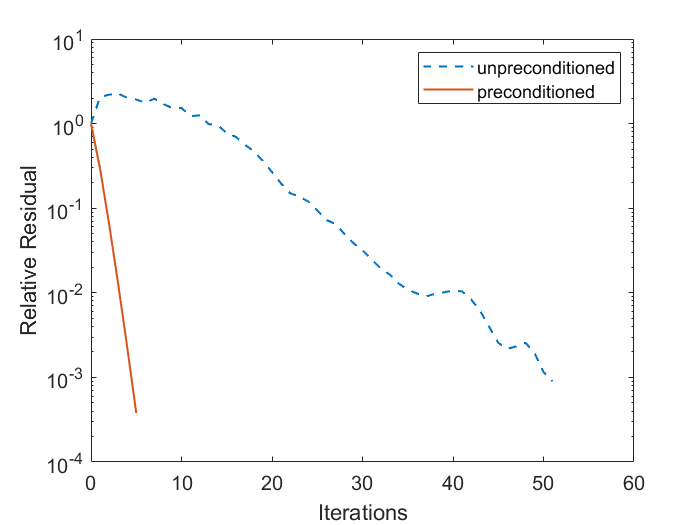
\includegraphics[height=6cm]{2_7_1.png}
    \caption{relative residual of CG and PCG }
  \end{figure}

  In Figure 1.1 the solid line is a plot of $\|r_k\|_2/\|b\|_2$
  for the preconditioned iteration and the dashed line for the
  unpreconditioned. Note that the unpreconditioned reduction in
  $\|r\|$ is not monotone. This is consistent  
  with the theory, which predicts decrese in $\|e\|_A$ but not
  necessarily in $\|r\|$ as the iteration progresses.
  
  \begin{figure}[H]
    \centering\label{fig:2.7.2}
    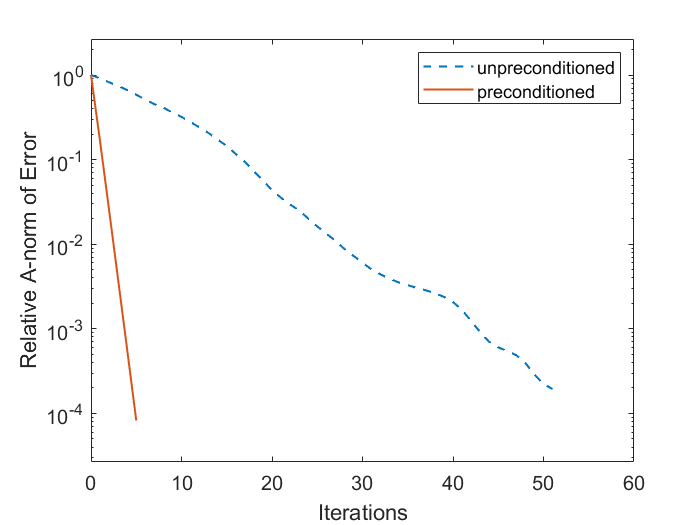
\includegraphics[height=6cm]{2_7_2.png}
    \caption{relative error of CG and PCG }
  \end{figure}
  
   In Figure 1.2 the solid line is a plot of $\|u^*-u_k\|_A/\|u^*-u_0\|_A$
  for the preconditioned iteration and the dashed line for the
  unpreconditioned.  The preconditioned iteration required 5
  iterations for convergence and the unpreconditioned iteration
  52. Note that the unpreconditioned iteration is slowly 
  convergent. This can be explained by the fact that the eigenvalues
  are not clustered and $$\kappa(A)=O(1/h^2)=O(n^2)=O(N).$$
\end{exm}

\subsection{CGNR and CGNE}
\label{sec:2.6}

\begin{defi}
  If $A$ is nonsingular and nonsymmetric, one might consider solving
  $Ax=b$ by applying CG to the normal equations
  \begin{equation}
    \label{eq:2.32}
    A^TAx=A^Tb.
  \end{equation}
  This approach is called CGNR.
\end{defi}

\begin{rmk}
  The reason for this name is that the minimization property of CG as
  applied to \eqref{eq:2.32} asserts that
  \begin{equation*}
    \begin{aligned}
      \|x^*-x\|^2_{A^TA}&=(x^*-x)^TA^TA(x^*-x) \\
      &=(Ax^*-Ax)^T(Ax^*-Ax)=\|r\|^2_2
    \end{aligned}
  \end{equation*}
  is minimized over $x_0+\mathcal{K}_k$ at each iterate. Hence it is
  called CG on the Normal equations to minimize the Residual.
\end{rmk}

\begin{defi}
  If $A$ is nonsingular and nonsymmetric, one could also consider
  applying CG to the normal equations
  \begin{equation}
    \label{eq:2.32}
    AA^Ty=b
  \end{equation}
  and then set $x=A^Ty$. This approach is called CGNE.
\end{defi}

\begin{rmk}
  The reason for this name is that the minimization property of CG as
  applied to \eqref{eq:2.32} asserts that
  \begin{equation*}
    \begin{aligned}
      \|y^*-y\|^2_{AA^T}&=(y^*-y)^TAA^T(y^*-y) \\
      &=(A^Ty^*-A^Ty)^T(A^Ty^*-A^Ty)\\&=\|x^*-x\|_2^2
    \end{aligned}
  \end{equation*}
  is minimized over $y_0+\mathcal{K}_k$ at each iterate. Hence it is
  called CG on the Normal equations to minimize the Error.
\end{rmk}

\begin{rmk}
  There are three  disadvantages that may or may not be serious:
  \begin{itemize}
  \item The condition number of $A^TA$ is the square of that of $A$.
  \item Two matrix-vector products are needed for each CG iterate
    since $\omega=A^T(Ap)$ in CGNR and $\omega=A(A^Tp)$ in CGNE.
  \item One must compute the action of $A^T$ on a vector as part of
    the matrix-vector product involving $A^TA$.
  \end{itemize}
\end{rmk}

%%% Local Variables:
%%% mode: latex
%%% TeX-master: "GMRES_MathDocument"
%%% End:

  

\section{GMRES Iteration}
\label{sec:3}

\subsection{The minimization property and its consequences}
\label{sec:3.1}

\begin{thm}[The minimization property of GMRES iteration]
  Let $A$ be nonsingular. The $k$th iteration of GMRES is the solution
  to the least squares
  problem
  \begin{equation}
    \label{eq:3.1}
    \text{minimize}_{x\in x_0+\mathcal{K}_k}\|b-Ax\|_2.
  \end{equation}
  Then for all $\overline{p}_k\in\mathcal{P}_k$
  \begin{equation}
    \label{eq:3.2}
    \|r_k\|_2=\min_{p\in\mathcal{P}_k}\|p(A)r_0\|_2\leq \|\overline{p}_k(A)r_0\|_2
  \end{equation}
\end{thm}

\begin{proof}
  Note that if $x\in x_0+\mathcal{K}_k$,
  then $$x=x_0+\sum\limits_{j=0}^{k-1}\gamma_{j}A^jr_0$$
  and so
  $$b-Ax=b-Ax_0-\sum\limits_{j=0}^{k-1}\gamma_{j}A^{j+1}r_0
  =r_0-\sum\limits_{j=1}^{k}\gamma_{j-1}A^jr_0$$
  Hence if $x\in x_0+\mathcal{K}_k$ then $r=\overline{p}(A)r_0$ where
  $\overline{p}\in\mathcal{P}_k$ is a residual polynomial, so
  \eqref{eq:3.2} is proved.
\end{proof}

\begin{coro}
  Let $A$ be nonsingular and let $x_k$ be the $k$th GMRES
  iteration. Then for all $\overline{p}_k\in\mathcal{P}_k$
  \begin{equation}
    \label{eq:3.3}
    \frac{\|r_k\|_2}{\|r_0\|_2}\leq \|\overline{p}_k(A)\|_2.
  \end{equation}
\end{coro}

\begin{thm}
  Let $A$ be nonsingular. Then the GMRES algorithm will find the
  solution within $N$ iterations.
\end{thm}

\begin{proof}
  The characteristic polynomial of $A$ is $p(z)=\det(A-zI)$. $p$ has
  degree $N$ and $p(0)=\det(A)\neq 0$ since $A$ is nonsingular, so
  $$\overline{p}_N(z)=p(z)/p(0)\in\mathcal{P}_N$$
  is a residual polynomial. It is well known that
  $p(A)=0=\overline{p}_N(A).$ By \eqref{eq:3.3}, $r_N=b-Ax_N=0$ and
  hence $x_N$ is the solution.
\end{proof}

\begin{thm}
  Let $A=V\Lambda V^{-1}$ be a nonsingular diagonalizable matrix. Let
  $x_k$ be the $k$th GMRES iterate. Then for all
  $\overline{p}_k\in\mathcal{P}_k$
  \begin{equation}
    \label{eq:3.4}
    \frac{\|r_k\|_2}{\|r_0\|_2}\leq \kappa_2(V)\max_{z\in\sigma(A)}|\overline{p}_k(z)|.
  \end{equation}
\end{thm}

\begin{proof}
  Let $\overline{p}_k\in\mathcal{P}_k.$ We can easily estimate
  $\|\overline{p}_k(A)\|_2$ by
  $$\|\overline{p}_k(A)\|_2\leq
  \|V\|_2\|V^{-1}\|_2\|\overline{p}_k(\Lambda)\|_2\leq
  \kappa_2(V)\max_{z\in\sigma(A)}|\overline{p}_k(z)|,$$
  as asserted.
\end{proof}

\begin{coro}
  If $A$ is normal, then we have
  $$\frac{\|r_k\|_2}{\|r_0\|_2}\leq\max_{z\in\sigma(A)}|\overline{p}_k(z)|.$$
\end{coro}

\begin{thm}
  Let $A$ be a nonsingular diagonalizable matrix. Assume that $A$ has
  only $k$ distinct eigenvalues. Then GMRES will terminate in at most
  $k$ iterations.
\end{thm}

\begin{thm}
  Let $A$ be a nonsingular normal matrix. Let $b$ be a linear
  combination of $k$ of the eigenvectors of $A$
  $$b=\sum\limits_{l=1}^k\gamma_lu_{i_l}.$$
  Then the GMRES iteration, with $x_0=0,$ for $Ax=b$ will terminate in
  at most $k$ iterations.
\end{thm}

\subsection{Termination}
\label{sec:3.2}

\begin{exm}
  Assume that $A=V\Lambda V^{-1}$ is diagonalizable, that the
  eigenvalues of $A$ lie in the interval $(9,11)$, and that
  $\kappa_2(V)=100$. We assume that $x_0=0$ and hence $r_0=b$. Using
  residual polynomial $\overline{p}_k(z)=(10-z)^k/10^k$ we find
  $$\frac{\|r_k\|_2}{\|r_0\|_2}\leq (100)10^{-k}=10^{2-k}.$$
  Hence
  \begin{equation}
    \label{eq:3.5}
    \|r_k\|_2\leq\eta\|b\|_2
  \end{equation}
  holds when $k>2+\log_{10}(\eta).$
\end{exm}

\begin{lemma}
  Assume that $A$ is nonsingular, diagonalizable and $\|I-A\|_2\leq \rho<1.$ Let
  $\overline{p}_k(z)=(1-z)^k.$
  We have
  \begin{equation}
    \label{eq:3.6}
    \|r_k\|_2\leq \rho^k\|r_0\|_2.
  \end{equation}
\end{lemma}

\begin{rmk}
  The estimate \eqref{eq:3.6} illustrates the potential benefits of a
  good approximate inverse precondition.
\end{rmk}

\subsection{Preconditioning}
\label{sec:3.3}

\begin{defi}
  If one can find $M$ such that $$\|I-MA\|_2=\rho<1,$$
  then applying GMRES to $MAx=Mb$ allows one to apply \eqref{eq:3.6}
  to the preconditioned system. Preconditioning done in this way is
  called \emph{left preconditioning}.
\end{defi}

\begin{rmk}
  If $r=MAx-Mb$ allows one to apply \eqref{eq:3.6} to the
  preconditioned system, we have
  $$\frac{\|e_k\|_2}{\|e_0\|_2}\leq
  \kappa_2(MA)\frac{\|r_k\|_2}{\|r_0\|_2}.$$
  If $MA$ has a smaller condition number than $A$, we might expect the
  relative residual of the preconditioned system to be a better
  indicator of the relative error than that of the original system.
\end{rmk}

\begin{defi}
    If one can find $M$ such that $$\|I-AM\|_2=\rho<1,$$
  one can solve $AMy=b$ with GMRES and then set $x=My.$
  This is called \emph{right preconditioning}.
\end{defi}

\begin{rmk}
  The residual of the preconditioned problem is the same as that of
  the unpreconditioned problem. Right preconditioning has been used as
  the basis for a method that changes the preconditioner as the
  iteration progresses.  
\end{rmk}

\subsection{Implementation: Basic ideas}
\label{sec:3.4}

\begin{lemma}
  The least squares problem defining the $k$th GMRES iterate,
  $$\text{minimize}_{x\in x_0+\mathcal{K}_k}\|b-Ax\|_2,$$
  is equivalent to the least squares problem in $\mathbb{R}^k$,
  \begin{equation}
    \label{eq:3.7}
    \text{minimize}_{y\in\mathbb{R}^k}\|r_0-AV_k y\|_2,
  \end{equation}
  where $V_k$ is an orthogonal projector onto $\mathcal{K}_k.$
\end{lemma}

\begin{proof}
  For any $z\in\mathcal{K}_k$, $z$ can be written
  as $$z=\sum\limits_{l=1}^ky_lv_l^k,$$
  where $v_l^k$ is the $l$th column of $V_k$. Hence we can convert
  \eqref{eq:3.1} to a least squares problem in $\mathbb{R}^k$ for the
  coefficient vector $y$ of $z=x-x_0$. Since $x-x_0=V_ky$ for some
  $y\in\mathbb{R}^k$, we must have $x_k=x_0+V_ky$ where $y$ minimizes
  \begin{equation*}
    \|b-A(x_0+V_ky)\|_2=\|r_0-AV_ky\|_2.\qedhere
  \end{equation*}
\end{proof}

\begin{rmk}
  We could solve this problem with a QR factorization. However, the
  problem is that the matrix vector product of $A$ with the basis matrix
  $V_k$ must be taken at each iteration. 
\end{rmk}

\begin{algo}
  The Gram-Schmit procedure for formation of an orthonormal basis for
  $\mathcal{K}_k$ is called the \emph{Arnoldi process}.
  
    \IncMargin{1em}
  \LinesNumbered
  \begin{algorithm}[H]
    \SetKwInOut{Precond}{Preconditions}
    \SetKwInOut{Postcond}{Postconditions}

    \caption{\texttt{Arnodi Process}}
    \KwIn{$x_0\in\mathbb{R}^n$, $b\in\mathbb{R}^n$, 
      $A\in\mathbb{R}^{N\times N}$,
    $k\in\mathbb{Z}^+$}
    \KwOut{Orthonormal basis for $\mathcal{K}_k$ stored in $V$}
    \BlankLine
    $r_0=b-Ax_0,\ v_1=r_0/\|r_0\|_2$\;
    \For{$i=1,\ldots,k-1$}{
      $v_{i+1}=\frac{Av_i-\sum_{j=1}^i((Av_i)^Tv_j)v_j}
      {\|Av_i-\sum_{j=1}^i((Av_i)^Tv_j)v_j\|_2}$
    }
  \end{algorithm}
  \DecMargin{1em}
\end{algo}

\begin{lemma}
  Let $A$ be nonsingular, let the vectors $v_j$ be generated by
  Algorithm \texttt{Arnoldi}, and let $i$ be the smallest integer for
  which
  $$Av_i-\sum_{j=1}^i((Av_i)^Tv_j)v_j=0.$$
  Then $x=A^{-1}b\in x_0+\mathcal{K}_i.$
\end{lemma}

\begin{proof}
  By hypothesis $Av_i\in\mathcal{K}_i$ and hence
  $A\mathcal{K}_i\subset\mathcal{K}_i.$ Since the columns of $V_i$ are
  an orthonormal basis for $\mathcal{K}_i,$ we have $$AV_i=V_iH,$$
  where $H$ is an $i\times i$ matrix. $H$ is nonsingular since $A$
  is. Setting $\beta=\|r_0\|_2$ and
  $e_1=(1,0,\ldots,0)^T\in\mathbb{R}^i$, we have
  $$\|r_i\|_2=\|b-Ax_i\|_2=\|r_0-A(x_i-x_0)\|_2.$$
  Since $x_i-x_0\in\mathcal{K}_i$ there is $y\in\mathbb{R}^i$ such
  that $x_i-x_0=V_iy.$ Since $r_0=\beta V_ie_1$ and $V_i$ is an
  orthogonal matrix
  $$\|r_i\|_2=\|V_i(\beta e_1-Hy)\|_2=\|\beta
  e_1-Hy\|_{\mathbb{R}^{i+1}},$$
  where $\|\cdot\|_{\mathbb{R}^{i+1}}$ denotes the Euclidean norm in
  $\mathbb{R}^{i+1}.$

  Setting $y=\beta H^{-1}e_1$ proves that $r_i=0$ by the minimization
  property. 
\end{proof}

\begin{lemma}
  The \texttt{Arnoldi process}(unless it terminates permaturely with a
  solution) produces matrices $\{V_k\}$ with orthonormal columns such
  that there exists an upper Hessenberg   matrix
  $H_k\in\mathbb{R}^{(k+1)\times k}$,
  \begin{equation}
    \label{eq:3.8}
    AV_k=V_{k+1}H_k
  \end{equation}
\end{lemma}

\begin{proof}
  Set $h_{ij}=(Av_j)^Tv_i$, it is easy to prove that $H_k$ is upper
  Hessenberg and \eqref{eq:3.8} holds. 
\end{proof}

\begin{coro}
  The least squares problem in the $k$th GMRES iterate is equivalent
  to the least squares problem in $\mathbb{R}^{k}$
  \begin{equation*}
    \text{minimize}_{y^k\in\mathbb{R}^k}\|\beta e_1-H_ky^k\|_{\mathbb{R}^{k+1}}.
  \end{equation*}
\end{coro}

\begin{proof}
  For some $y^k\in\mathbb{R}^k$,
  $$r_k=b-Ax_k=r_0-A(x_k-x_0)=V_{k+1}(\beta e_1-H_ky^k).$$
  Hence $x_k=x_0+V_ky^k$, where $y^k$ minimizes $\|\beta e_1-H_ky\|_2$
  over $\mathbb{R}^k$.

  Note that when $y^k$ has been computed, the norm of $r_k$ can be
  found without explicitly forming $x_k$ and computing $b-Ax_k$. We
  have
  \begin{equation} 
    \label{eq:3.9}
    \begin{split}
      \|r_k\|_2&=\|V_{k+1}(\beta e_1-H_ky^k)\|_2\\
      &=\|\beta e_1-H_ky^k\|_{\mathbb{R}^{k+1}}. \qedhere
    \end{split}
  \end{equation}
\end{proof}

\begin{algo}
  The usual implementation of GMRES iteration reflects
  all of the above results.

  \IncMargin{1em}
  \LinesNumbered
  \begin{algorithm}[H]
    \SetKwInOut{Precond}{Preconditions}
    \SetKwInOut{Postcond}{Postconditions}

    \caption{\texttt{GMRESa}}
    \KwIn{$x\in\mathbb{R}^n$, $b\in\mathbb{R}^n$, 
      $A\in\mathbb{R}^{N\times N}$,
      $\epsilon\in\mathbb{R}^+, k_{\text{max}}\in\mathbb{Z}^+$}
    \KwOut{The solution which overwrites $x$, the residual norm $\rho$.}
    \Postcond{$\rho\leq\epsilon\|b\|_2$ or $k=k_{\text{max}}$} 
    \BlankLine
    $r=b-Ax,\ v_1=r/\|r\|_2,\ \rho=\|r\|_2^2$\;
    $k=0,\ \beta=\rho$\;
    \While{$\rho>\epsilon\|b\|_2$ and
      $k<k_{\text{max}}$}{
      $k=k+1$\;
      \For{$j=1,\ldots,k$}{
        $h_{jk}=(Av_k)^Tv_j$\;
      }
      $v_{k+1}=Av_k-\sum_{j=1}^kh_{jk}v_j$\;
      $h_{k+1,k}=\|v_{k+1}\|_2$\;
      $v_{k+1}=v_{k+1}/\|v_{k+1}\|_2$\;
      $e_1=(1,0,\ldots,0)^T\in\mathbb{R}^{k+1}$\;
      Minimize $\|\beta e_1-H_ky^k\|_{\mathbb{R}^{k+1}}$ over
      $\mathbb{R}^k$ to obtain $y^k$\;
      $\rho=\|\beta e_1-H_ky^k\|_{\mathbb{R}^{k+1}}$\;
    }
    $x_k=x_0+V_ky^k$\;
  \end{algorithm}
  \DecMargin{1em}
\end{algo}

\begin{rmk}
  \label{sec:impl-basic-ideas}
  Note that $x_k$ is only computed upon termination and is not needed
  within the iteration. It is an important property of GMRES that the
  basis for the Krylov space must be stored as the iteration progress.
\end{rmk}

\begin{defi}
  For very large problems, one way to avoid the problem in
  Remark \ref{sec:impl-basic-ideas}  is to set $k_{\text{max}}$ to the
  maximum number $m$ of vectors that one can store, call GMRES and
  explicitly test the residual $b-Ax_k$ if $k=m$ upon termination. If
  the norm of the residual is larger than $\epsilon$, call GMRES again
  with $x_0=x_k$.

  The restarted version of the algorithm is called \emph{GMRES(m)}.
\end{defi}

\begin{exm}
  Let $\delta=10^{-7}$ and define
  $$A=\left(
    \begin{array}{ccc}
      1&1&1 \\ \delta&\delta&0 \\ \delta & 0 & \delta
    \end{array}\right).
  $$
  We orthogonalize the columns of $A$ with classical Gram-Schmidt to
  obtain
  $$V=\left(
    \begin{array}{ccc}
      1.0000e+00 &1.0436e-07 & 9.9715e-08 \\
      1.0000e-07 & 1.0456e-14 & -9.9905e-01 \\
      1.0000e-07 & -1.0000e+00& 4.3568e-02
    \end{array}\right).
  $$
  The columns of $V$ are not orthogonal at all. In fact
  $v_2^Tv_3\approx -0.004.$

\end{exm}

\begin{algo}
  A partial remedy is to replace the classical Gram-Schmidt
  orthogonalization in Algorithm \texttt{GMRESa} with modified
  Gram-Schmidt orthogonalization.

  \IncMargin{1em}
  \LinesNumbered
  \begin{algorithm}[H]
    \SetKwInOut{Precond}{Preconditions}
    \SetKwInOut{Postcond}{Postconditions}

    \caption{\texttt{GMRESb}}
    \KwIn{$x\in\mathbb{R}^n$, $b\in\mathbb{R}^n$, 
      $A\in\mathbb{R}^{N\times N}$,
      $\epsilon\in\mathbb{R}^+, k_{\text{max}}\in\mathbb{Z}^+$}
    \KwOut{The solution which overwrites $x$, the residual norm $\rho$.}
    \Postcond{$\rho\leq\epsilon\|b\|_2$ or $k=k_{\text{max}}$} 
    \BlankLine
    $r=b-Ax,\ v_1=r/\|r\|_2,\ \rho=\|r\|_2^2$\;
    $k=0,\ \beta=\rho$\;
    \While{$\rho>\epsilon\|b\|_2$ and
      $k<k_{\text{max}}$}{
      $k=k+1$\;
      $v_{k+1}=Av_k$\;
      \For{$j=1,\ldots,k$}{
        $h_{jk}=(v_{k+1})^Tv_j$\;
        $v_{k+1}=v_{k+1}-h_{jk}v_j$\;
      }
      $h_{k+1,k}=\|v_{k+1}\|_2$\;
      $v_{k+1}=v_{k+1}/\|v_{k+1}\|_2$\;
      $e_1=(1,0,\ldots,0)^T\in\mathbb{R}^{k+1}$\;
      Minimize $\|\beta e_1-H_ky^k\|_{\mathbb{R}^{k+1}}$ over
      $\mathbb{R}^k$ to obtain $y^k$\;
      $\rho=\|\beta e_1-H_ky^k\|_{\mathbb{R}^{k+1}}$\;
    }
    $x_k=x_0+V_ky^k$\;
  \end{algorithm}
  \DecMargin{1em}
\end{algo}

\begin{exm}
  We take the same matrix $A$ as that in Example 1.3.19, for modified
  Gram-Schmidt, we have
  $$V=\left(
    \begin{array}{ccc}
      1.0000e+00 &1.0436e-07 & 1.0436e-07 \\
      1.0000e-07 & 1.0456e-14 & -1.0000e+00 \\
      1.0000e-07 & -1.0000e+00& 4.3565e-16
    \end{array}\right).
  $$
  Hence $|v_i^Tv_j-\delta|\leq 10^{-8}$ for all $i,j$.
\end{exm}

\begin{rmk}
  Even if modified Gram-Schmidt orthogonalization is used, one can
  still lose orthogonality in the columns of $V$. Reorthogonalization is
  necessary if $A$ is ill conditioned. One easy way is to augment the
  modified Gram-Schmidt process with a second pass. The implementation
  of reorthogonalization will be given in the end of the section.
\end{rmk}

\begin{rmk}
  The $k$th GMRES iteration requires a matrix-vector product, $k$
  scalar products, and the solution of the Hessenberg least problem in
  line 13. If we solve this problem by QR factorization, then the
  total cost of the $m$ GMRES iterations is $O(m^4).$ 
\end{rmk}

\subsection{Implementatin: Givens rotations}
\label{sec:3.5}

\begin{defi}
  A $2\times 2$ \emph{Givens rotation} is a matrix of the form
  \begin{equation}
    \label{eq:3.12}
    G=\left(
      \begin{array}{cc}
        c & -s \\ s & c
      \end{array}
    \right),
  \end{equation}
  where $c=\cos(\theta),\ s=\sin(\theta)$ for $\theta\in[-\pi,\pi]$.
\end{defi}

\begin{lemma}
  The $2\times 2$ Givens rotation rotates the vector $(c,-s)$, which
  makes an angle of $-\theta$ with the $x$-axis through an angle
  $\theta$ so that it overlaps the $x$-axis.
  $$
  G\left(
    \begin{array}{c}
      c \\ -s
    \end{array}
  \right)=\left(
    \begin{array}{c}
      0 \\ 1
    \end{array}
  \right).$$
\end{lemma}

\begin{defi}
  An $N\times N$ Givens rotation replaces a $2\times 2$ block on the
  diagonal of the $N\times N$ identity matrix with a $2\times 2$
  Givens rotation.
  \begin{equation}
    \label{eq:3.13}
    G=\left(
      \begin{array}{ccccccc}
        1 &0 & &\cdots & & & 0\\
        0 &\ddots &\ddots & & & & \\
          & \ddots& c&-s & & & \\
         \vdots & &s &c &0 & & \vdots\\
          & & & 0&1 &\ddots & \\
          & & & &\ddots &\ddots &0 \\
         & & &\cdots & &0 &1 
      \end{array}
    \right)
  \end{equation}
  $G_{j}(c,s)$ is an $N\times N$ Givens rotation of the form
  \eqref{eq:3.13} with a $2\times 2$ Givens rotation in rows and
  columns $j$ and $j+1$.
\end{defi}

\begin{lemma}
  Let $H$ be an $N\times M\ (N\geq M)$ upper Hessenberg matrix with
  rank $M$. There exists a product of Givens rotations $Q$ such that
  $QH=R$ is upper triangular.
\end{lemma}

\begin{proof}
  We reduce $H$ to triangular form by first multiplying the matrix by
  a Givens rotation that annihilates $h_{21}$ (and of course, changes
  $h_{11}$ and the subsequent columns). We define $G_1=G_1(c_1,s_1)$
  by
  \begin{equation}
    \label{eq:3.14}
    c_1=h_{11}/\sqrt{h_{11}^2+h_{21}^2}\ \text{and } s_1=-h_{21}/\sqrt{h_{11}^2+h_{21}^2}.
  \end{equation}
  If we replace $H$ by $G_1H$, then the first column of $H$ now has
  only a single nonzero element $h_{11}$. Similary we can now apply
  $G_2(c_2,s_2)$ to $H$, where
  \begin{equation}
    \label{eq:3.15}
    c_2=h_{22}/\sqrt{h_{22}^2+h_{32}^2}\ \text{and } s_2=-h_{32}/\sqrt{h_{22}^2+h_{32}^2}.
  \end{equation}
  and annihilate $h_{32}$. Note that $G_2$ does not affect the first
  column of $H$. Continuing in this way and setting $$Q=G_N\ldots
  G_1,$$
  we see that $QH=R$ is upper triangular.
\end{proof}

\begin{lemma}
  The least squares problem
  $$\text{minimize}_{y^k\in\mathbb{R}^k}\|\beta
  e_1-H_ky^k\|_{\mathbb{R}^{k+1}}$$
  is equivalent to the least squares problem in $\mathbb{R}^k$
  $$\text{minimize}_{y^k\in\mathbb{R}^k}\|g-R_ky^k\|_{\mathbb{R}^{k+1}}$$
  where $R_k$ is the $k+1\times k$ triangular factor of the QR
  factorization of $H_k$ and $g=\beta Qe_1$.
\end{lemma}


\begin{algo}
  The complete GMRES iteration reflects all of the above results.

  \IncMargin{1em}
  \LinesNumbered
  \begin{algorithm}[H]
    \SetKwInOut{Precond}{Preconditions}
    \SetKwInOut{Postcond}{Postconditions}

    \caption{\texttt{GMRES}}
    \KwIn{$x\in\mathbb{R}^n$, $b\in\mathbb{R}^n$, 
      $A\in\mathbb{R}^{N\times N}$,$\delta\in\mathbb{R}^{+}$,
      $\epsilon\in\mathbb{R}^+, k_{\text{max}}\in\mathbb{Z}^+$}
    \KwOut{The solution which overwrites $x$, the residual norm $\rho$.}
    \Postcond{$\rho\leq\epsilon\|b\|_2$ or $k=k_{\text{max}}$} 
    \BlankLine
    $r=b-Ax,\ v_1=r/\|r\|_2,\ \rho=\|r\|_2^2$\;
    $k=0,\ \beta=\rho$\;
    $g=\rho(1,0,\ldots,0)^T\in\mathbb{R}^{k_{\text{max}}+1}$\;
    \While{$\rho>\epsilon\|b\|_2$ and
      $k<k_{\text{max}}$}{
      $k=k+1$\;
      $v_{k+1}=Av_k$\;
      \For{$j=1,\ldots,k$}{
        $h_{jk}=(v_{k+1})^Tv_j$\;
        $v_{k+1}=v_{k+1}-h_{jk}v_j$\;
      }
      \If{$\|Av_k\|_2+\delta\|v_{k+1}\|_2=\|Av_k\|_2$}{
        \For{$j=1,\ldots,k$}{
          $h_{tmp}=(v_{k+1})^Tv_j$\;
          $h_{jk}=h_{jk}+h_{tmp}$\;
          $v_{k+1}=v_{k+1}-h_{tmp}v_j$\;
        }
      }
      $h_{k+1,k}=\|v_{k+1}\|_2$\;
      $v_{k+1}=v_{k+1}/\|v_{k+1}\|_2$\;
      \If{$k>1$}{
        apply $Q_{k-1}$ to the $k$th column of $H$\;
      }
      $\nu=\sqrt{h_{k,k}^2+h_{k+1,k}^2}$\;
      $c_k=h_{k,k}/\nu,\ s_k=-h_{k+1,k}/\nu$\;
      $h_{k,k}=c_kh_{k,k}-s_kh_{k+1,k},\ h_{k+1,k}=0$\;
      $g=G_k(c_k,s_k)g$\;
      $\rho=|(g)_{k+1}|$\;
    }
    Set $r_{i,j}=h_{i,j}$ for $1\leq i,j\leq k$\;
    Set $(\omega)_i=(g)_i$ for $1\leq i\leq k$\;
    Solve the upper triangular system $Ry^k=\omega$\;
    $x_k=x_0+V_ky^k$\;
  \end{algorithm}
  \DecMargin{1em}
\end{algo}

\begin{rmk}
  The cost of one single GMRES iteration is $O(N)$ floating-point
  operations. The $O(N^2)$ cost of the triangular solve and the $O(N)$
  cost of the construction of $x_k$ are incurred after
  termination. Hence the total cost of the $m$ GMRES iterations is $O(m^2)$.
\end{rmk}

\subsection{Examples for GMRES iteration}
\label{sec:3.7}

\begin{exm}
  We consider the discretization of the PDE
  \begin{equation}
    \label{eq:3.33}
    \begin{aligned}
      (Lu)(x,y)&=-(u_{xx}(x,y)+u_{yy}(x,y))+a_1(x,y)u_x(x,y)\\
      &+a_2(x,y)u_y(x,y)+a_3(x,y)u(x,y)=f(x,y)
      \end{aligned}
    \end{equation}
    on $0<x,y<1$ subject to homogeneous Dirichlet boundary conditions
    $$u(x,0)=u(x,1)=u(0,y)=u(1,y)=0,\ \ 0<x,y<1.$$
    For the computations reported in this section we took
    $$a_1(x,y)=1,\ a_2(x,y)=20y,\ a_3(x,y)=1.$$
    As before we discretize with a five-point centered difference
    scheme with $n^2$ points and mesh width $h=1/(n+1)$. Then let $n=31$ to
    create a system with 961 unknowns. As a preconditioner we use the
    fast Poisson solver, let $Gu$ denote the action of the Poisson
    solver on $u$, the preconditioned system is $GLu=Gf$.

   We take $u_0=0$ be the initial iterate and the right hand side so
   that the exact solution is the discretization of
   $$10xy(1-x)(1-y)\exp(x^{4.5})$$

   In Figure 1.3 we plot iteration histories corresponding to
   preconditioned and unpreconditioned GMRES.

    \begin{figure}[H]
    \centering\label{fig:3.7.1}
    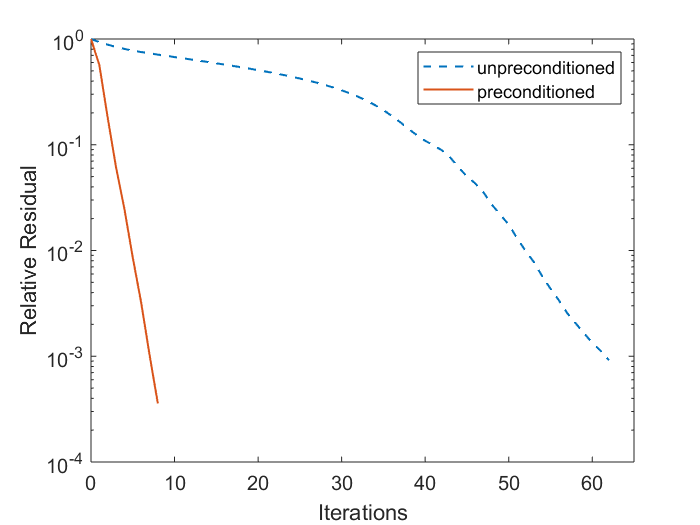
\includegraphics[height=6cm]{3_7_1.png}
    \caption{relative residual of PGMRES and GMRES.}
  \end{figure}
\end{exm}
%%% Local Variables:
%%% mode: latex
%%% TeX-master: "GMRES_MathDocument"
%%% End:



\end{multicols}
\end{document}
%%% Local Variables:
%%% mode: latex
%%% TeX-master: t
%%% End:
